% !TeX root = ../report.tex
\chapter{Grundlagen}

Im vorliegenden Bericht wird vielseitig auf praktische Aspekte die zum Bau eines Passivradars notwendig sind eingegangen. Um dem Leser das Verständnis dieser Aspekte zu erleichtern, ist es sinnvoll, zunächst die theoretischen Grundlagen zu erläutern. Dieses Kapitel dient der Beschreibung einiger essenzieller Prinzipien, die bei Passivradar zum Einsatz kommen. Dazu wird zunächst der Begriff der bistatischen Geometrie eingeführt und erklärt, anschließend wird diese im Zusammenhang mit passiver Zieldetektion und -lokalisierung kombiniert und mit einer mathematischen Beschreibung versehen. Schließlich wird auf konstruktionsabhängige Eigenarten, sowie Vor- und Nachteile eingegangen.

\section{Bistatische Geometrie}

In der Ortungstechnik versteht man unter dem Begriff der bistatischen Geometrie die räumliche Trennung zwischen einem Sender und einem Empfänger. Dies lässt sich für Systeme mit mehreren Sendern und Empfängern verallgemeinern und wird dann auch als multistatisches System bezeichnet. Im umgekehrten Fall, nämlich dann wenn die räumliche Trennung zwischen Sender und Empfänger als vernachlässigbar klein verstanden wird, spricht man von monostatischen Systemen. Die Abbildung~\ref{fig:mono_bi_multistatic_geometry} zeigt vereinfachte Illustrationen dieser Konzepte. Tx und Rx bezeichnen hierbei jeweils Sender und Empfänger im System.

\begin{figure}[htb]
    \centering
    \subcaptionbox{Monostatische Geometrie.\label{fig:monostatic_geometry}}{
        \begin{tikzpicture}
            \node at (0,0) [draw,fill=white] (radar) {Tx \& Rx};

            \node [label={above:Ziel}] (target) at (2,2) {\Huge\faPlane};

            \draw [<->,red] (radar) -- (target);
        \end{tikzpicture}
    }
    \subcaptionbox{Bistatische Geometrie.\label{fig:bistatic_geometry}}{
        \begin{tikzpicture}
            \coordinate (rx1_coord) at (-1,0);
            \coordinate (tx1_coord) at (2,0);
            \coordinate (target_coord) at (1.75,1.5);

            \node at (tx1_coord) [draw,fill=white] (tx1) {Tx};
            \node at (rx1_coord) [draw,fill=white] (rx) {Rx};

            \node at (target_coord) [label={above:Ziel}] (target) {\Large\faPlane};

            \draw [->,color=red] (tx1) -- (target);
            \draw [->,color=red] (target) -- (rx);
            \draw [->,color=blue] (tx1) -- (rx);
        \end{tikzpicture}
    }
    \subcaptionbox{Multistatische Geometrie.\label{fig:multistatic_geometry}}{
        \begin{tikzpicture}
            \coordinate (rx1_coord) at (-2,1);
            \coordinate (rx2_coord) at (-1,-0.5);
            \coordinate (tx1_coord) at (3,0);
            \coordinate (tx2_coord) at (2,-1);
            \coordinate (target_coord) at (2,2);

            \node at (tx1_coord) [draw,fill=white] (tx1) {Tx 1};
            \node at (tx2_coord) [draw,fill=white] (tx2) {Tx 2};
            \node at (rx1_coord) [draw,fill=white] (rx1) {Rx 1};
            \node at (rx2_coord) [draw,fill=white] (rx2) {Rx 2};

            \node at (target_coord) [label={above:Ziel}] (target) {\Large\faPlane};

            \draw [->,color=red] (tx1) -- (target);
            \draw [->,color=red] (tx2) -- (target);
            \draw [->,color=red] (target) -- (rx1);
            \draw [->,color=red] (target) -- (rx2);
            \draw [->,color=blue] (tx1) -- (rx1);
            \draw [->,color=blue] (tx1) -- (rx2);
            \draw [->,color=blue] (tx2) -- (rx1);
            \draw [->,color=blue] (tx2) -- (rx2);
        \end{tikzpicture}
    }

    \caption{Mono-, Bi- und Multistatische Geometrie.}\label{fig:mono_bi_multistatic_geometry}
\end{figure}

\section{Passive Zieldetektion und -lokalisierung}

\section{Bauarten}

\section{Vor- und Nachteile}
